% Compilar desde report/ con:
%   xelatex -interaction=nonstopmode informe_final_eryndor.tex
%   xelatex -interaction=nonstopmode informe_final_eryndor.tex
\documentclass[11pt]{article}

\usepackage[letterpaper,margin=0.82in]{geometry}
\usepackage{fontspec}
\usepackage{xcolor}
\usepackage{graphicx}
\usepackage{amsfonts}
\usepackage{booktabs}
\usepackage{tabularx}
\usepackage{longtable}
\usepackage{array}
\usepackage{enumitem}
\usepackage{float}
\usepackage{hyperref}

\setmainfont[
  Path=../presentation/fonts/,
  BoldFont=FreeSansBold.ttf,
  ItalicFont=FreeSansOblique.ttf
]{FreeSans.ttf}

\definecolor{Obsidian}{HTML}{171A24}
\definecolor{DeepPurple}{HTML}{2B1E3E}
\definecolor{CosmicBlue}{HTML}{4A4E8F}
\definecolor{MineralCyan}{HTML}{4FC3C8}
\definecolor{EmberGold}{HTML}{D6A34A}
\definecolor{Lavender}{HTML}{A490C2}
\definecolor{Moss}{HTML}{79A879}
\definecolor{Paper}{HTML}{F7F5FA}
\definecolor{Ink}{HTML}{272432}

\hypersetup{
  colorlinks=true,
  linkcolor=CosmicBlue,
  urlcolor=CosmicBlue,
  citecolor=DeepPurple,
  pdftitle={Eryndor: Guardianes del Velo},
  pdfauthor={Pablo Daniel Barillas Moreno y Wilson Alejandro Calderón}
}
\Urlmuskip=0mu plus 1mu\relax

\graphicspath{{../artifacts/dataset/}{../artifacts/phase8/}{../artifacts/gallery/}}
\setlength{\parindent}{0pt}
\setlength{\parskip}{0.58em}
\setlist[itemize]{leftmargin=1.35em,itemsep=0.25em,topsep=0.25em}
\setlist[enumerate]{leftmargin=1.55em,itemsep=0.25em,topsep=0.25em}
\renewcommand{\arraystretch}{1.2}

\makeatletter
\renewcommand\section{\@startsection{section}{1}{\z@}%
  {-3.2ex \@plus -1ex \@minus -.2ex}%
  {1.6ex \@plus .2ex}%
  {\normalfont\Large\bfseries\color{DeepPurple}}}
\renewcommand\subsection{\@startsection{subsection}{2}{\z@}%
  {-2.8ex \@plus -1ex \@minus -.2ex}%
  {1.1ex \@plus .2ex}%
  {\normalfont\large\bfseries\color{CosmicBlue}}}
\makeatother
\pagestyle{plain}

\newcommand{\metric}[2]{%
  \begin{minipage}[t]{0.22\textwidth}
    \colorbox{Paper}{\parbox[c][0.75in][c]{0.94\linewidth}{\centering
      {\scriptsize\color{CosmicBlue}\MakeUppercase{#1}}\\[3pt]
      {\Large\bfseries\color{DeepPurple}#2}}}
  \end{minipage}
}

\newcommand{\callout}[2]{%
  \noindent\colorbox{Paper}{\parbox{0.96\linewidth}{\vspace{5pt}
  \textbf{\color{#1}#2}\vspace{5pt}}}
}

\begin{document}

\begin{titlepage}
\pagecolor{Obsidian}
\color{white}
\vspace*{0.65in}
{\small\bfseries\color{MineralCyan}\MakeUppercase{Deep Learning 2026 · Proyecto 2}}\\[0.35in]
{\fontsize{34}{38}\selectfont\bfseries Eryndor}\\[0.08in]
{\fontsize{25}{30}\selectfont Guardianes del Velo}\\[0.28in]
{\large\color{Lavender}Diseño generativo de personajes para un RPG pixel art de aventura y magia}

\vfill
\colorbox{DeepPurple}{\parbox[c][1.65in][c]{0.91\textwidth}{\hspace{0.28in}\begin{minipage}{0.83\textwidth}
\textbf{Universidad del Valle de Guatemala}\\
Deep Learning · Sección 30\\[0.16in]
\textbf{Integrantes}\\
Pablo Daniel Barillas Moreno\\
Wilson Alejandro Calderón\\[0.16in]
\textbf{Repositorio}\\
\href{https://github.com/DanielBarillasM/Proyecto-2_Grupo-1_DLYSI_Sec-30.git}{github.com/DanielBarillasM/Proyecto-2\_Grupo-1\_DLYSI\_Sec-30}
\end{minipage}}}

\vfill
{\small\color{Lavender}Informe final reproducible · GAN entrenada por el equipo · Sin imágenes finales de generadores externos}
\end{titlepage}
\nopagecolor
\color{Ink}

\section*{Resumen ejecutivo}

Este proyecto estudia si una GAN entrenada sobre sprites abiertos y visualmente consistentes puede generar personajes plausibles, diversos y defendibles como nuevos dentro del universo de Eryndor. Se construyó un dataset determinista de 4,096 imágenes RGB de $64\times64$ píxeles a partir de recursos Liberated Pixel Cup, con cero archivos faltantes, cero hashes duplicados y atribución resuelta para las 254 capas utilizadas.

Se entrenaron tres variantes DCGAN durante 60 épocas bajo un protocolo controlado: BCE base, hinge loss y BCE con normalización espectral en el discriminador. Hinge sufrió colapso de modo; la variante con normalización espectral mantuvo la mayor diversidad final y fue seleccionada. A partir de 200 candidatos se eligieron diez mediante una regla pre-registrada de calidad, novedad y diversidad. Los diez PNG son únicos, tienen vectores latentes persistidos y regeneran con diferencia RGB máxima igual a cero.

\begin{center}
\metric{Dataset}{4,096}\hfill
\metric{Entrenamiento}{60/60}\hfill
\metric{Selección}{10/200}\hfill
\metric{Delta RGB}{0}
\end{center}

\tableofcontents
\newpage

\section{Problema, universo y criterio de éxito}

La pregunta central fue: \emph{¿puede una GAN entrenada sobre sprites abiertos y consistentes generar personajes de Eryndor que sean plausibles, diversos y distintos de sus vecinos más cercanos en entrenamiento?}

Eryndor es un mundo de fantasía fracturado por la Ruptura Celeste. La magia se solidifica en minerales luminosos y sus guardianes recorren fortalezas derruidas, bosques húmedos y observatorios olvidados para cerrar grietas arcanas. El lenguaje visual usa pixel art detallado, cuerpo completo, perspectiva ortográfica elevada, materiales gastados y una paleta oscura con acentos cian, oro y amatista.

El éxito exigía: código regenerable; diez personajes distintos; evolución visible con ruido fijo; ausencia de copias exactas frente al entrenamiento; comparación de experimentos cambiando una sola variable; y trazabilidad desde checkpoint y vector $z$ hasta cada PNG.

\section{Dataset, procedencia y preparación}

\subsection{Fuente y licencias}

Las composiciones derivan del \emph{Universal LPC Spritesheet Character Generator}. El commit fijado fue:

\begin{center}
\small\texttt{4963a69795255fb15a934c47f478a8bdcf3668f5}
\end{center}

LPC integra activos bajo licencias abiertas como CC0, CC-BY, CC-BY-SA, OGA-BY y GPL. El repositorio conserva autores, licencias y URL por capa en \path{docs/LPC_CREDITS_USED.csv}; se resolvieron 254 de 254 créditos.

\subsection{Pipeline reproducible}

La semilla de dataset fue \texttt{2026}. El pipeline aplicó composición alfa de cuerpo, ropa, cabello, accesorios y armas; extrajo la pose frontal de $64\times64$; fijó un fondo obsidiana; y calculó SHA-256 sobre píxeles RGB antes de aceptar cada imagen. El resultado fue:

\begin{itemize}
  \item 4,096 imágenes RGB, cero faltantes y cero hashes duplicados;
  \item 2,060 cuerpos \texttt{male} y 2,036 \texttt{female};
  \item 44 estilos de cabello y 18 estilos de torso;
  \item ocupación media de primer plano de 23.18\%, con rango 16.04\%--31.57\%;
  \item lotes \texttt{float32} de forma $[64,3,64,64]$ normalizados a $[-1,1]$.
\end{itemize}

\begin{figure}[H]
  \centering
  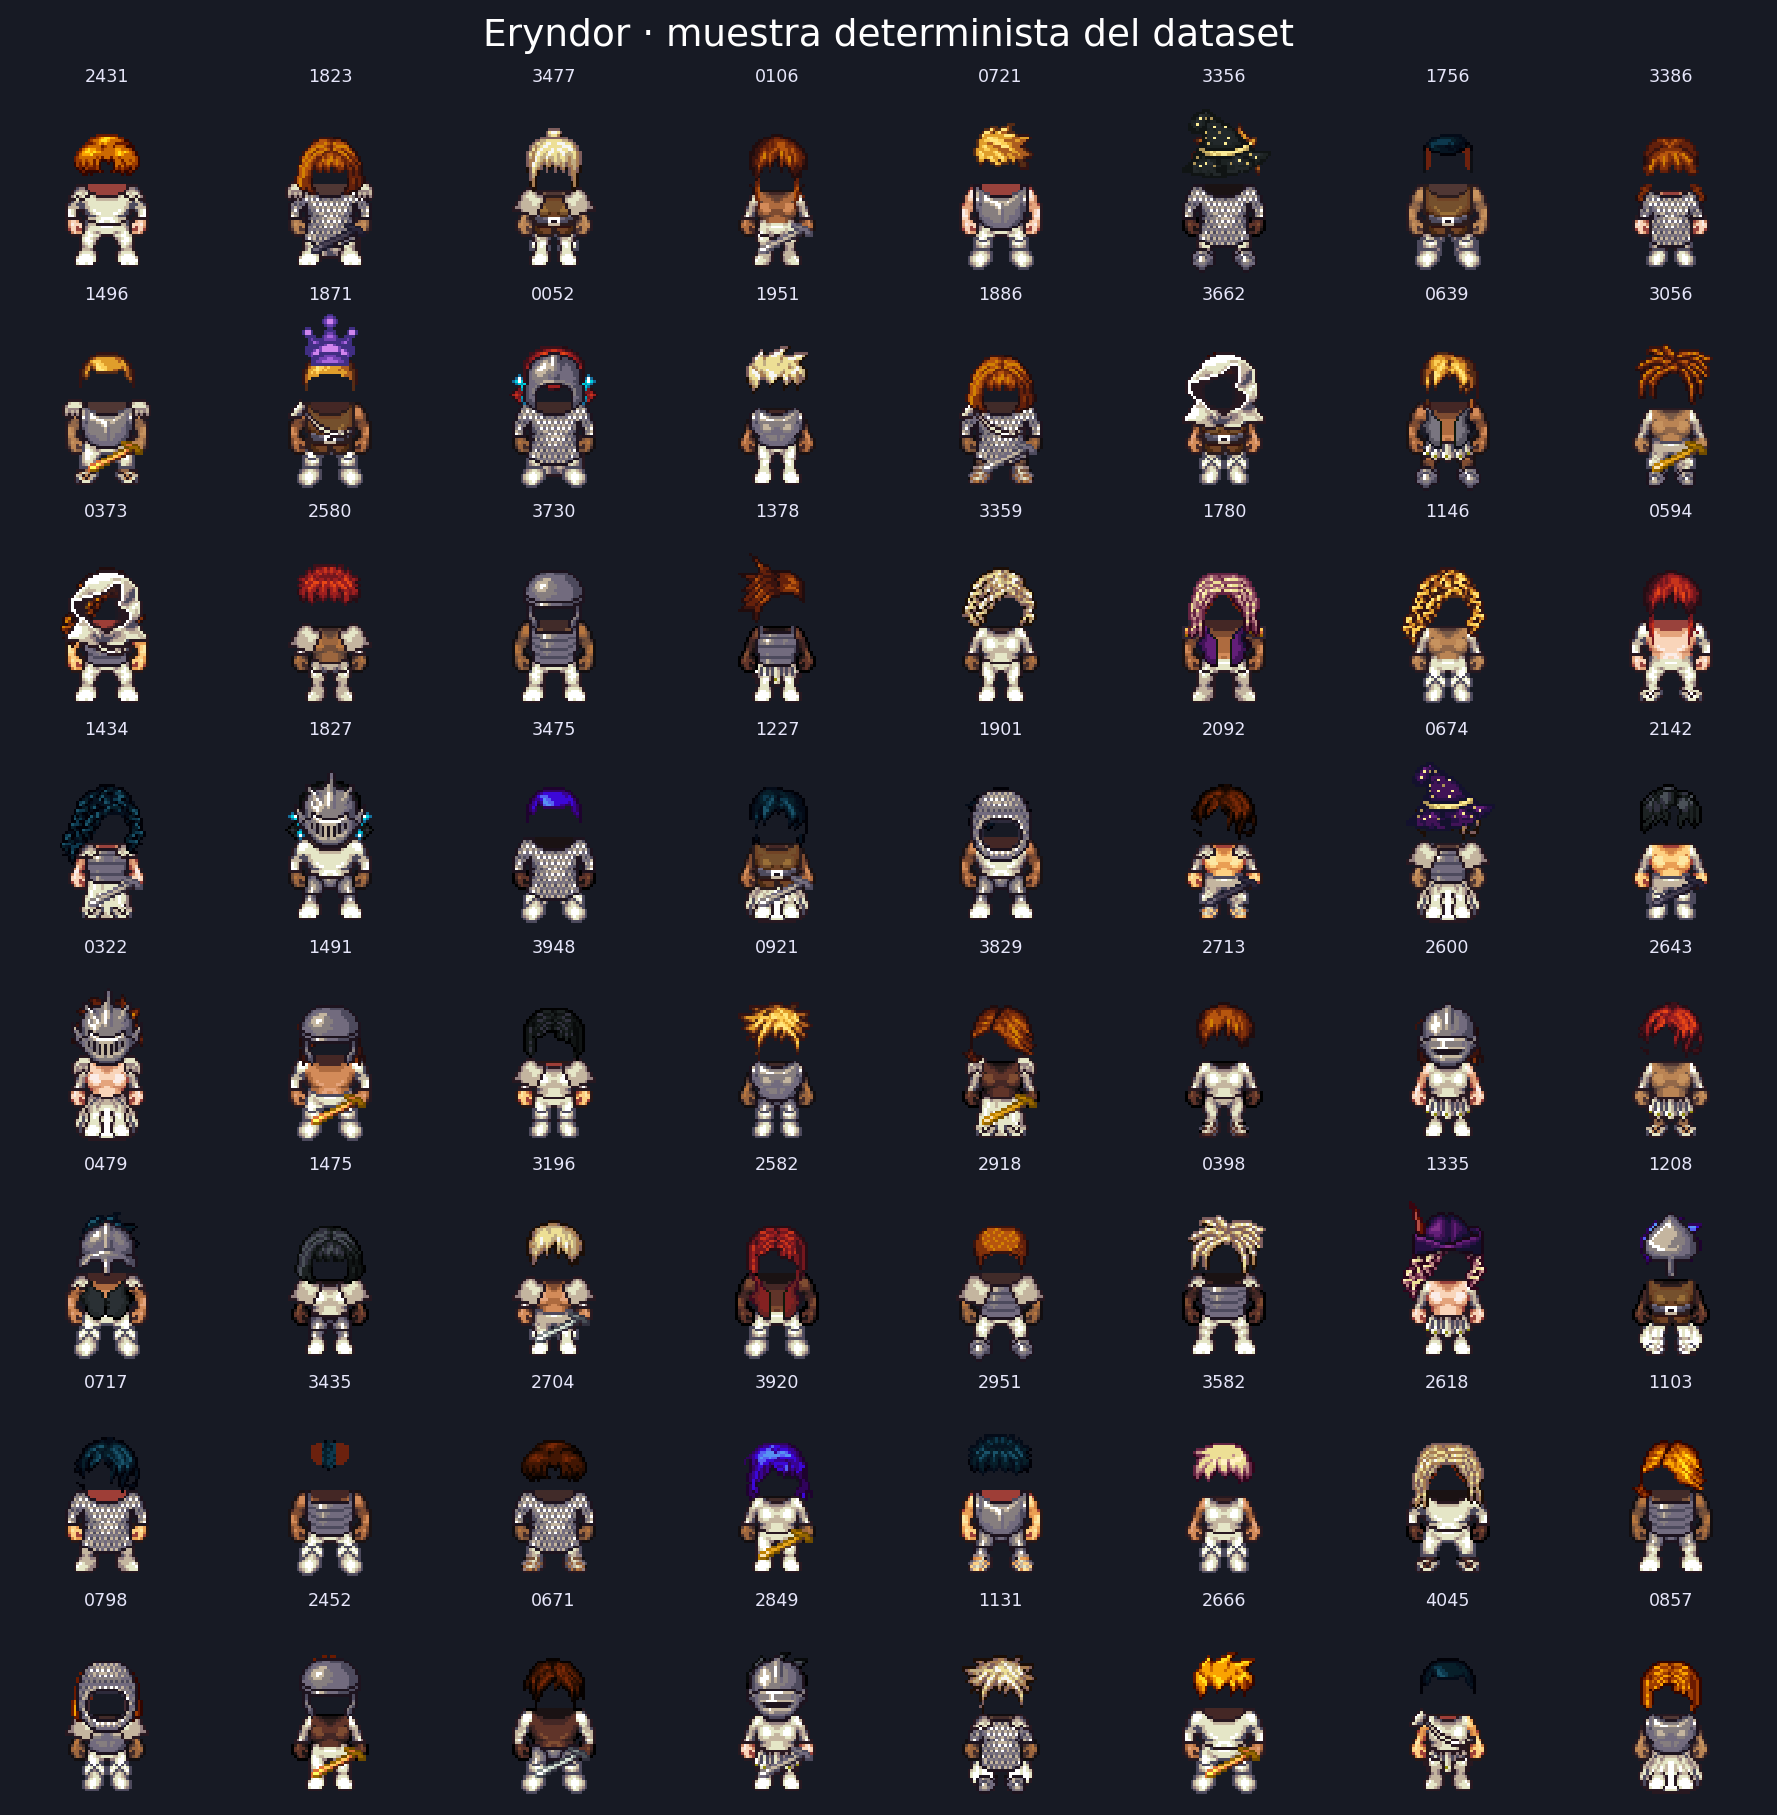
\includegraphics[width=0.88\textwidth]{dataset_contact_sheet.png}
  \caption{Muestra determinista del dataset preparado.}
\end{figure}

\callout{EmberGold}{Limitación del corpus. El dataset es composicional, comparte bases anatómicas y contiene una sola pose frontal. Esto favorece control visual y legal, pero limita la diversidad estructural que la GAN puede aprender.}

\section{Arquitectura y protocolo experimental}

El generador proyecta $z\in\mathbb{R}^{128}$ desde $1\times1$ hasta una imagen RGB de $64\times64$ mediante cinco convoluciones transpuestas, BatchNorm, ReLU y salida \texttt{tanh}. El discriminador reduce la imagen a un logit escalar con cinco convoluciones, LeakyReLU 0.2 y BatchNorm desde el segundo bloque. El generador contiene 3,806,080 parámetros y el discriminador 2,765,568.

Se eligió DCGAN porque el corpus es homogéneo y tiene resolución fija de $64\times64$, la arquitectura cabe en los recursos de Google Colab y permite aislar el efecto de la pérdida y de la estabilización sin cambiar simultáneamente el modelo. Es una elección de control y trazabilidad experimental, no una afirmación de estado del arte.

La configuración común fue batch 64, Adam con $lr=2\times10^{-4}$, $\beta_1=0.5$, $\beta_2=0.999$, semilla de modelo \texttt{42}, ruido fijo \texttt{777}, 60 épocas y checkpoints reanudables.

\begin{table}[H]
\centering
\caption{Experimentos controlados y pre-registrados.}
\begin{tabularx}{\textwidth}{@{}l l l X@{}}
\toprule
ID & Pérdida & Estabilización & Hipótesis y criterio previo \\
\midrule
A & BCE no saturante & Baseline & Creemos que BCE producirá siluetas reconocibles porque el dataset es consistente. Lo consideraremos útil si el ruido fijo progresa sin converger a una apariencia. \\
B & Hinge & Igual a A & Creemos que hinge mejorará rasgos porque mantiene gradientes útiles. Lo consideraremos útil si mejora calidad y diversidad sin acercarse al entrenamiento. \\
C & BCE no saturante & Spectral norm en D & Creemos que normalización espectral estabilizará a D porque limita sus capas. Lo consideraremos útil si reduce su dominio y sostiene el ruido fijo. \\
\bottomrule
\end{tabularx}
\end{table}

Solo cambió la pérdida en B y la estabilización en C. Datos, arquitectura, semillas, optimizadores, épocas y ruido fijo permanecieron iguales.

\section{Resultados de entrenamiento}

Los tres experimentos completaron 60 épocas. La auditoría consolidó 180 registros por época y 11,520 pasos sin duplicados, faltantes ni valores no finitos.

\begin{table}[H]
\centering
\caption{Métricas de la época final.}
\begin{tabular}{@{}lrrrrr@{}}
\toprule
Experimento & $L_D$ & $L_G$ & Logit real & Logit falso G & Diversidad \\
\midrule
BCE base & 0.0789 & 5.6369 & 5.1900 & $-5.6287$ & 0.2585 \\
Hinge & 0.0000 & 8.1271 & 5.0046 & $-8.1271$ & 0.0136 \\
BCE + spectral norm & 0.1905 & 7.0557 & 5.4518 & $-7.0458$ & \textbf{0.2659} \\
\bottomrule
\end{tabular}
\end{table}

Las escalas de BCE y hinge no son directamente comparables. La interpretación combinó la trayectoria de cada variante, los mismos 16 vectores fijos, diversidad y revisión visual. Hinge acumuló 23 épocas con $L_D<10^{-3}$ y terminó con diversidad 0.0136, evidencia de colapso. BCE base produjo personajes reconocibles. C sostuvo la mayor diversidad final, 0.2659, y la mayor media de las últimas diez épocas, 0.2671; por ello se convirtió en el modelo final y luego fue confirmado por las auditorías de fases 9--11.

\begin{figure}[H]
  \centering
  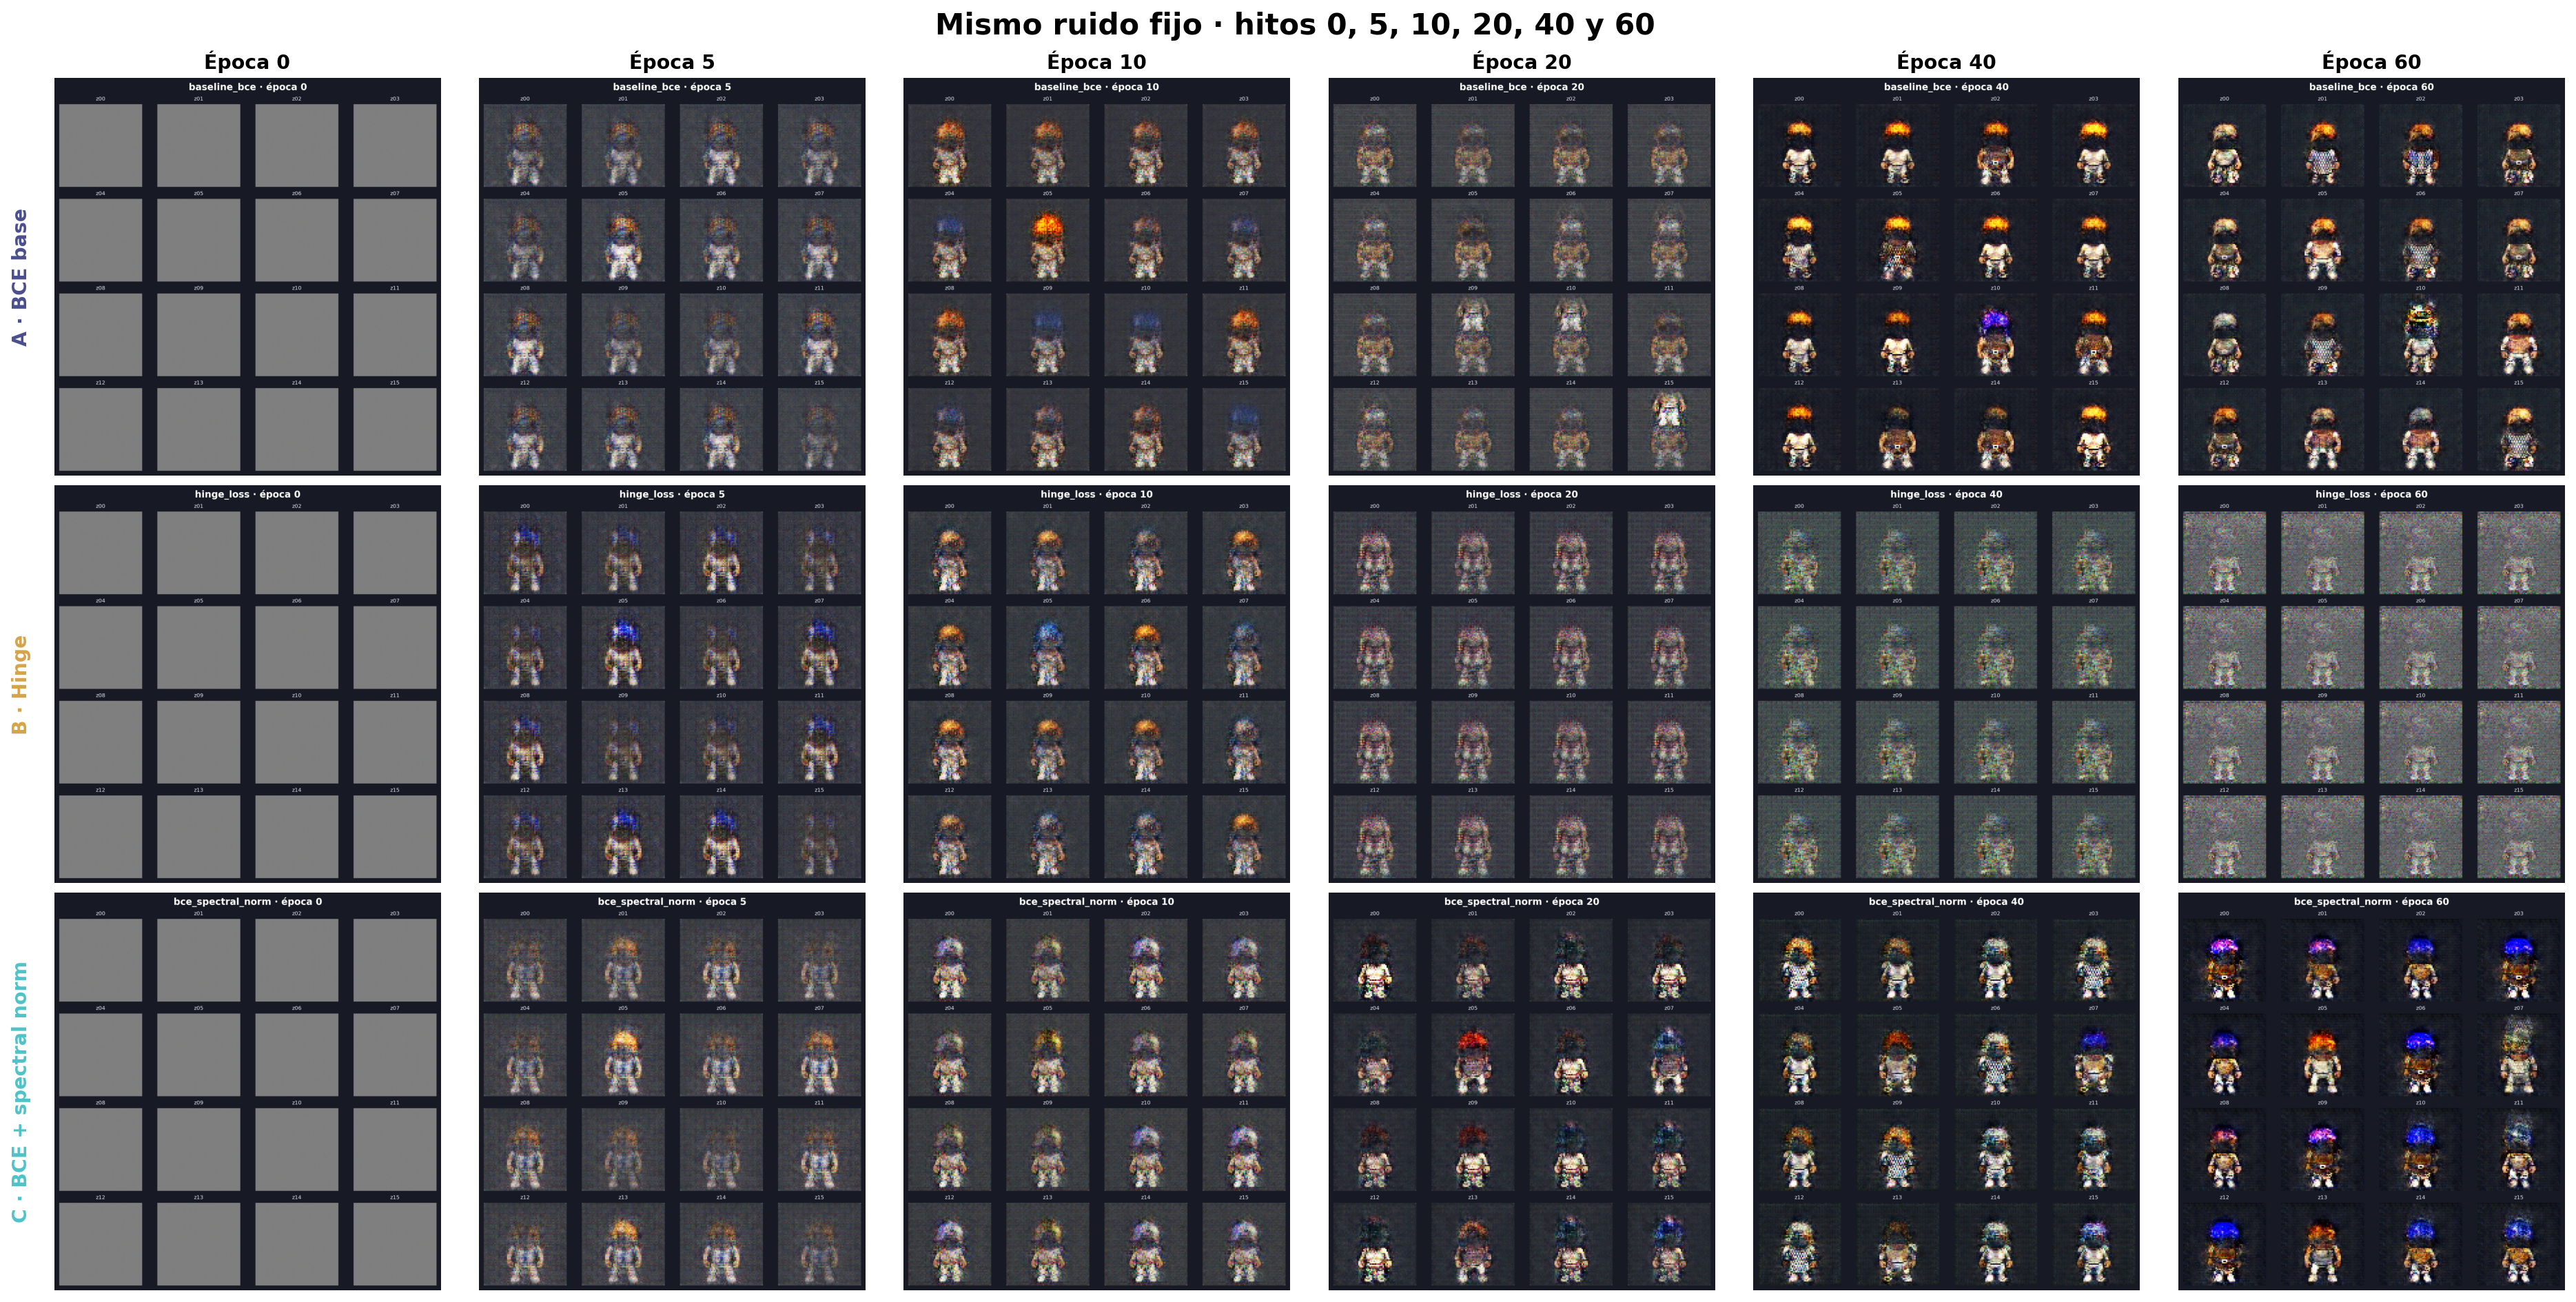
\includegraphics[width=\textwidth]{fixed_noise_milestones.png}
  \caption{Los mismos 16 vectores de ruido en épocas 0, 5, 10, 20, 40 y 60.}
\end{figure}

\begin{figure}[H]
  \centering
  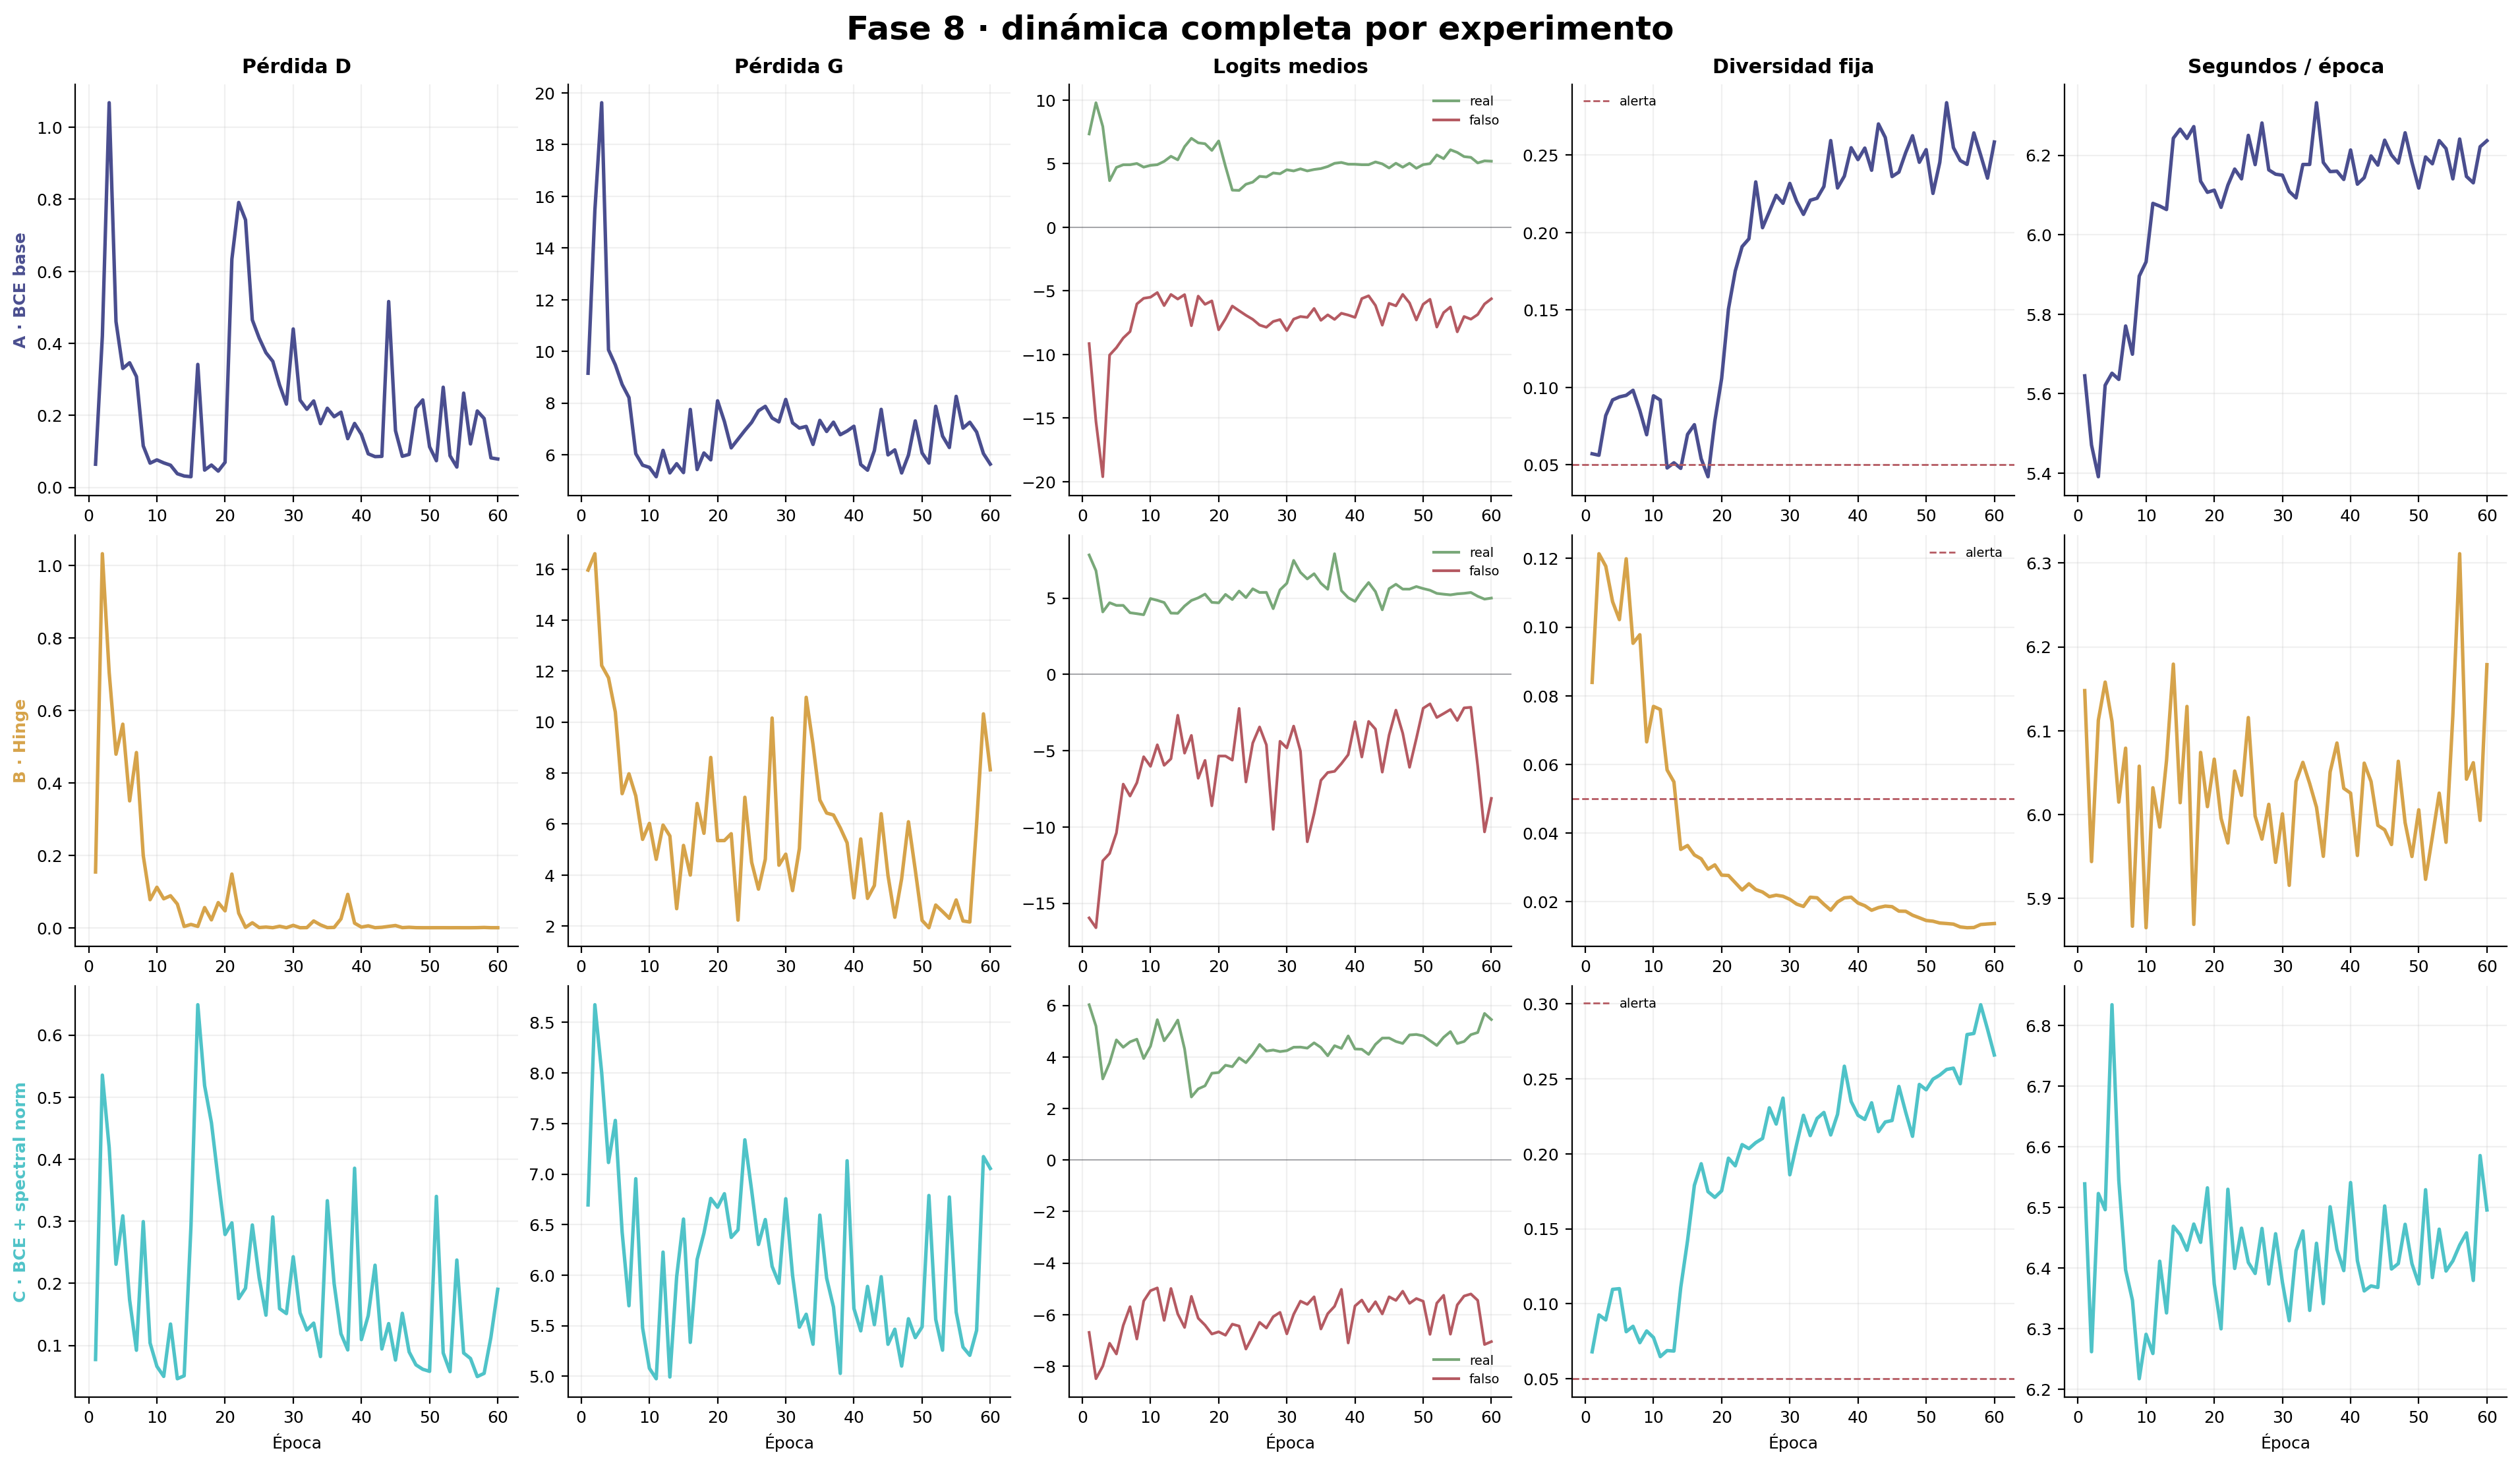
\includegraphics[width=0.95\textwidth]{phase8_diagnostics.png}
  \caption{Pérdidas, logits y diversidad de las trayectorias completas.}
\end{figure}

\section{Novedad, selección y galería final}

\subsection{Auditoría de vecinos}

La fase 9 comparó 16 muestras de ruido fijo contra las 4,096 imágenes reales mediante ResNet18 IMAGENET1K\_V1 sin capa final, similitud coseno y MSE. El coseno medio fue 0.7660; el MSE medio, 0.02615. No se encontraron duplicados exactos ni casos que cumplieran simultáneamente la bandera de revisión $\mathrm{coseno}\geq0.95$ y $\mathrm{MSE}\leq0.01$.

\subsection{Selección transparente}

Con semilla \texttt{20261011}, el modelo final generó 200 candidatos. Los límites técnicos de ocupación y contraste se derivaron del dataset. Noventa y siete candidatos fueron elegibles. El primero se eligió con 70\% novedad y 30\% calidad; los nueve restantes, con 55\% diversidad interna, 30\% novedad y 15\% calidad. No hubo sustitución manual. La tasa declarada fue $10/200=5\%$.

Los índices seleccionados fueron 100, 35, 144, 141, 114, 15, 48, 20, 0 y 39. Su coseno medio frente al vecino real fue 0.7563 y el MSE medio 0.02152.

\begin{figure}[H]
  \centering
  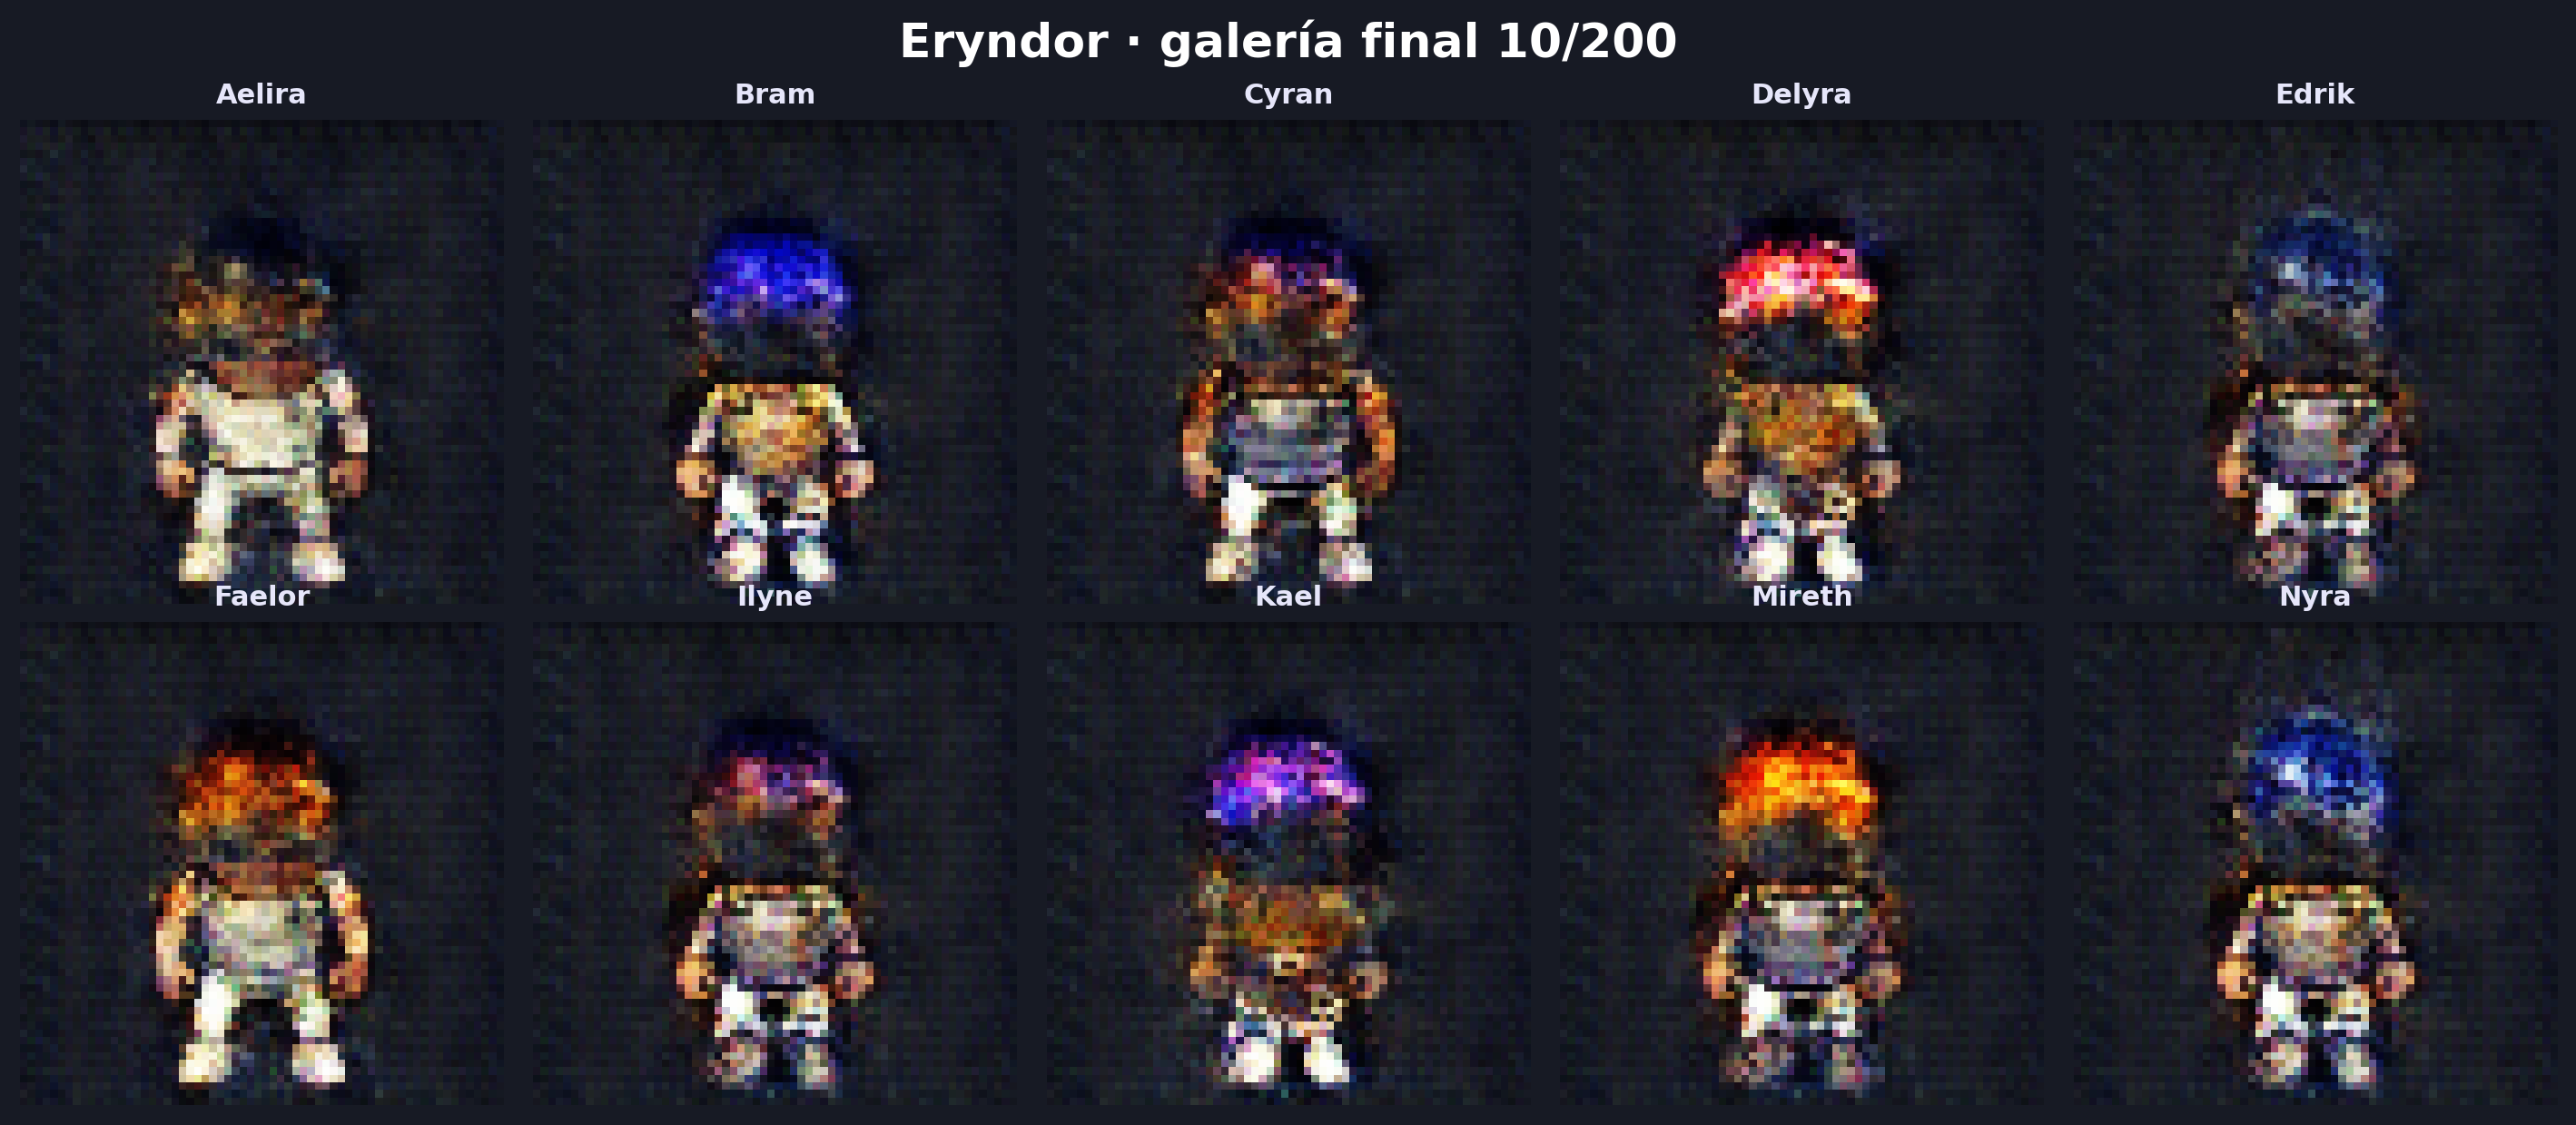
\includegraphics[width=\textwidth]{final_gallery_grid.png}
  \caption{Galería final de diez personajes generados por la GAN del equipo.}
\end{figure}

\begin{longtable}{@{}r l p{4.2cm} r r r@{}}
\caption{Personajes y métricas frente al vecino real.}\\
\toprule
\# & Nombre & Rol & Candidato & Coseno & MSE \\
\midrule
\endfirsthead
\toprule
\# & Nombre & Rol & Candidato & Coseno & MSE \\
\midrule
\endhead
1 & Aelira & Oráculo del Velo & 100 & 0.6981 & 0.01489 \\
2 & Bram & Guardián rúnico & 35 & 0.7911 & 0.01485 \\
3 & Cyran & Arcanista de ceniza & 144 & 0.7676 & 0.03245 \\
4 & Delyra & Exploradora del musgo & 141 & 0.7593 & 0.02025 \\
5 & Edrik & Alquimista solar & 114 & 0.7449 & 0.02029 \\
6 & Faelor & Centinela de amatista & 15 & 0.7660 & 0.03430 \\
7 & Ilyne & Tejedora de grietas & 48 & 0.7426 & 0.01655 \\
8 & Kael & Custodio de la brasa & 20 & 0.7482 & 0.01530 \\
9 & Mireth & Cartógrafa astral & 0 & 0.7804 & 0.02499 \\
10 & Nyra & Vigía del abismo & 39 & 0.7644 & 0.02135 \\
\bottomrule
\end{longtable}

\begin{figure}[H]
  \centering
  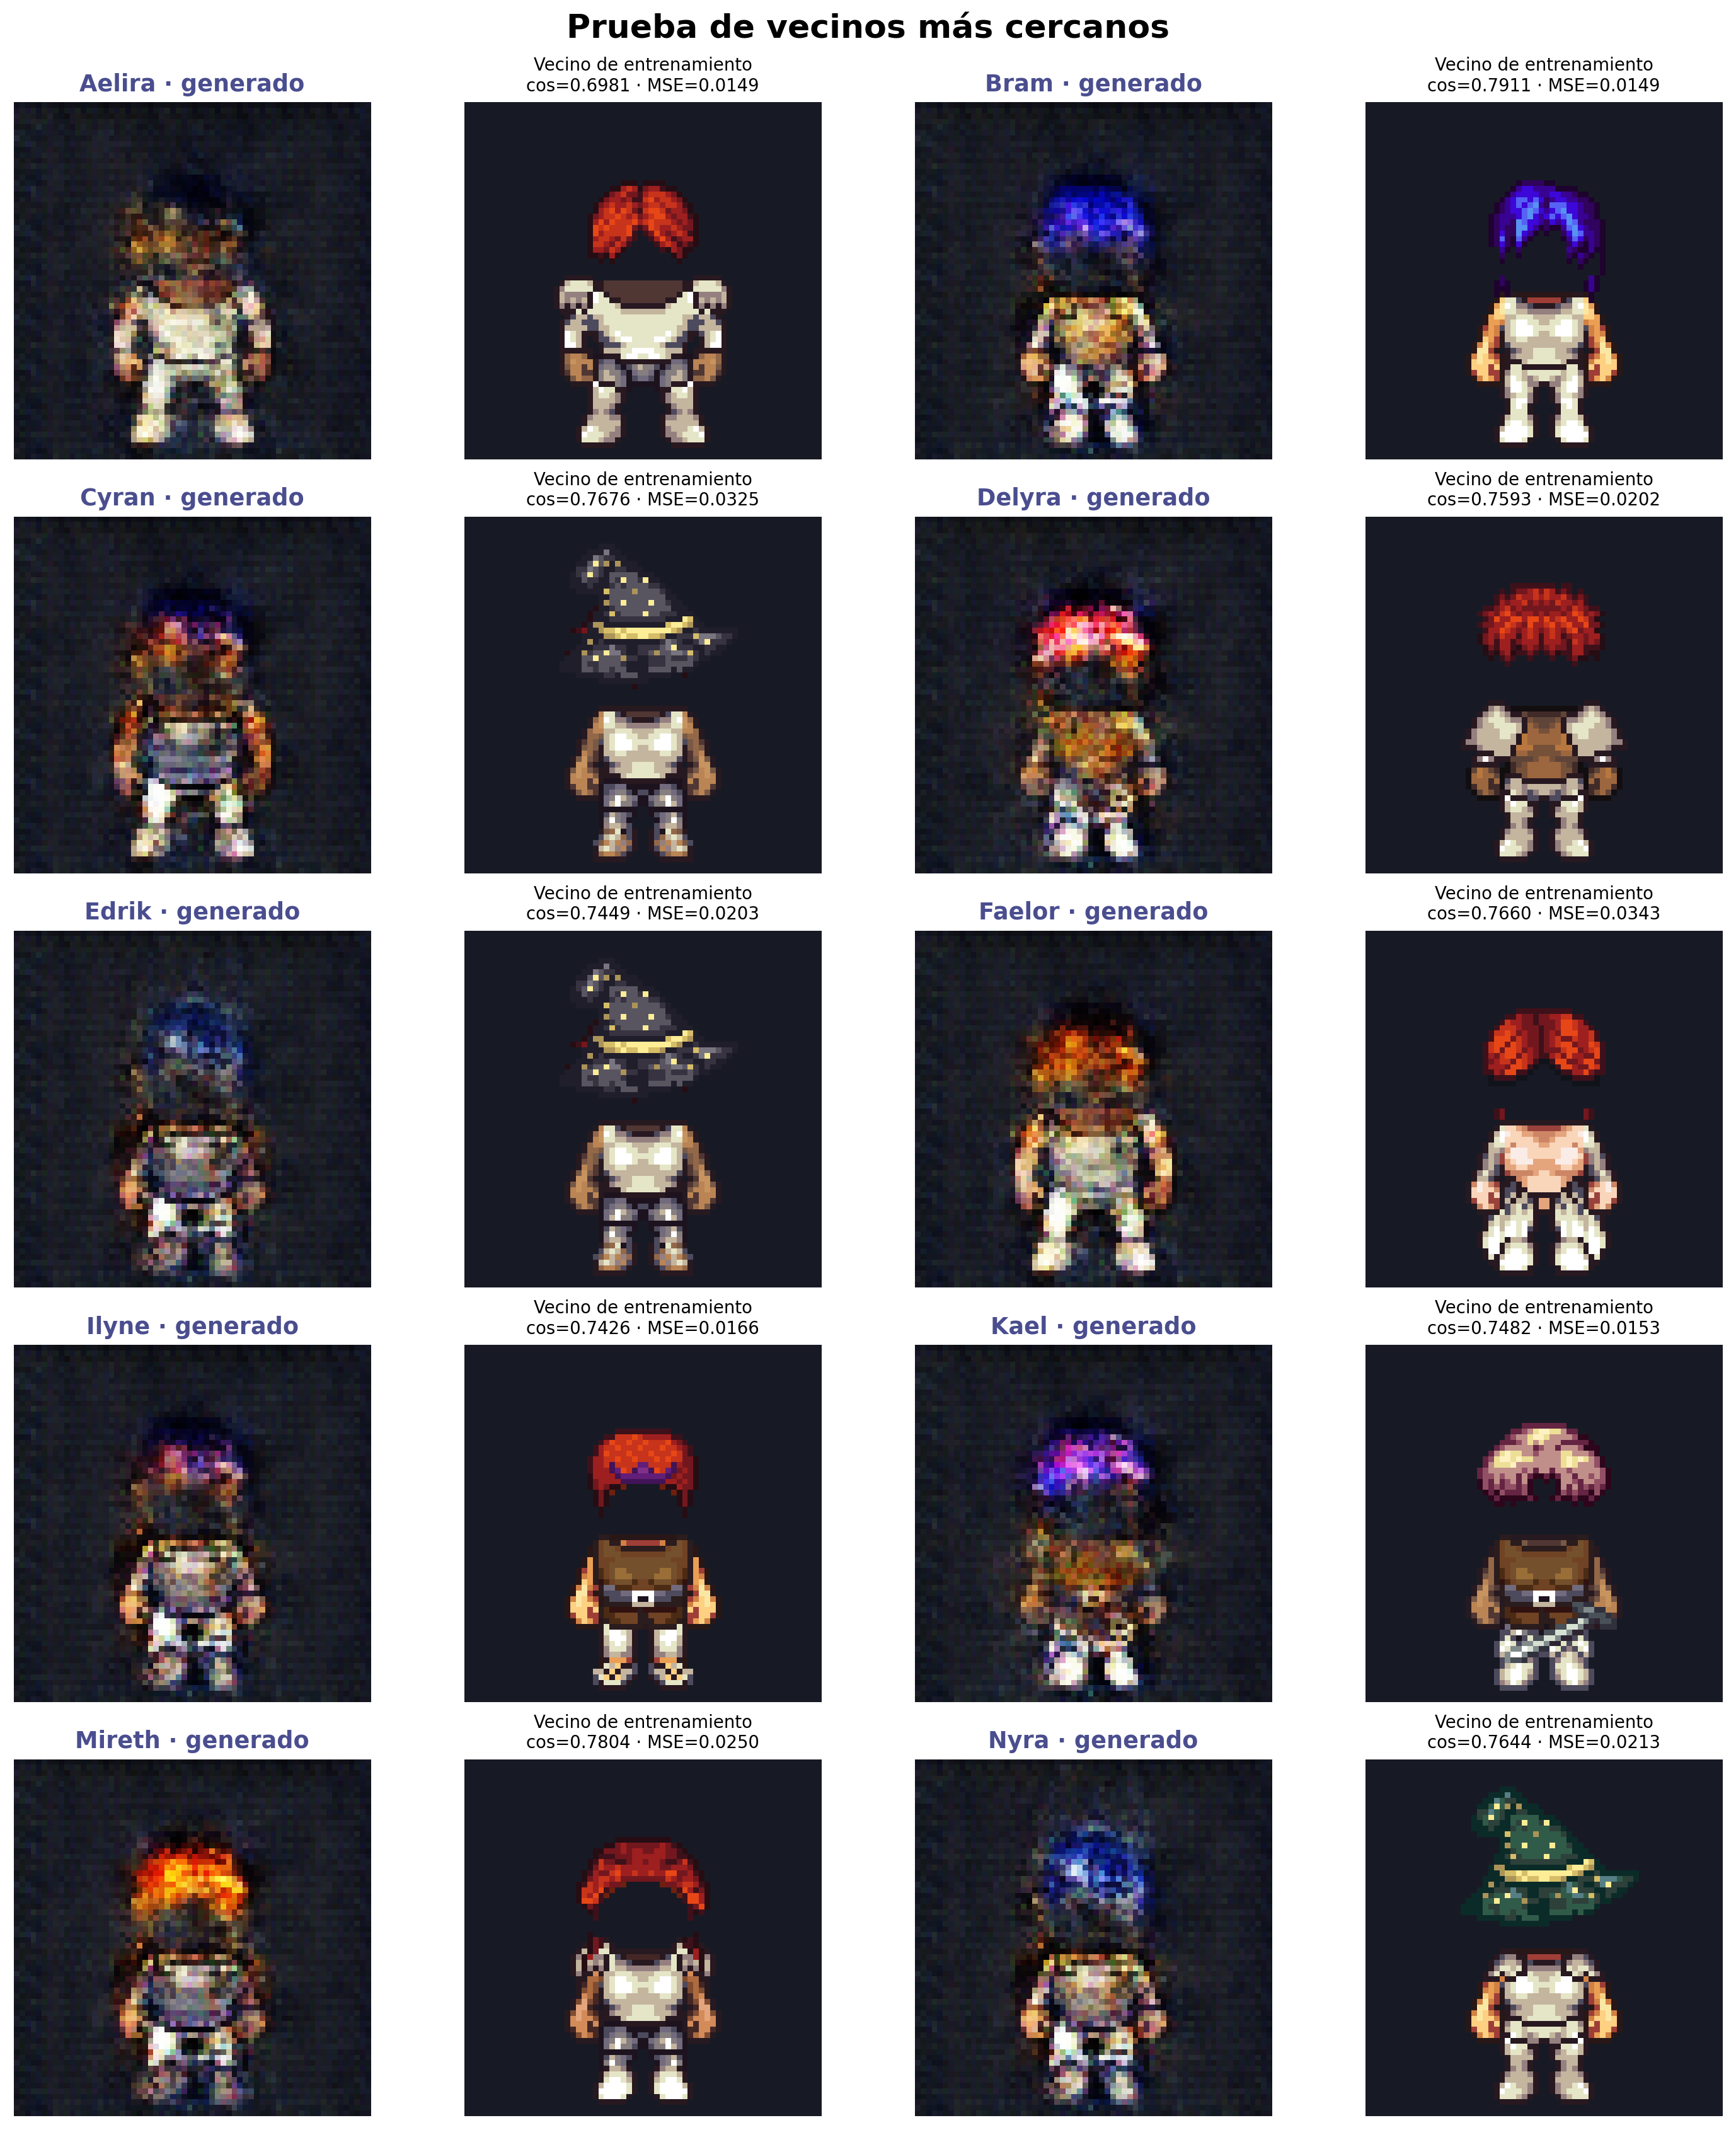
\includegraphics[width=0.9\textwidth]{nearest_neighbors.png}
  \caption{Cada personaje final junto a su vecino más cercano del entrenamiento.}
\end{figure}

\subsection{Reflexión final}

\textbf{Bram, Guardián rúnico}, es el personaje más difícil de defender como nuevo porque alcanza el mayor coseno, 0.7911, frente a su vecino real; su MSE es 0.01485. Comparte la silueta global, la pose y parte de la gramática cromática del conjunto, aunque la composición generada no es una copia exacta.

Este caso muestra que la GAN aprendió bien la gramática frontal restringida de LPC y recombinó atributos superficiales. También revela el límite del aprendizaje: con una única pose y anatomías compartidas, la diversidad estructural es reducida incluso cuando no existe duplicación exacta.

\section{Reproducibilidad y trazabilidad}

Cada PNG final se vincula con su vector $z$, índice de candidato, semilla, SHA-256, checkpoint, vecino real y métricas en \texttt{galeria/manifest.csv}. \texttt{galeria/latents.npz} tiene forma $[10,128,1,1]$. La selección coincide con fase 10, los diez hashes son únicos y la regeneración desde checkpoint produce diferencia RGB máxima igual a cero.

El código, notebooks y artefactos versionados se encuentran en el \href{https://github.com/DanielBarillasM/Proyecto-2_Grupo-1_DLYSI_Sec-30.git}{\textbf{repositorio GitHub del proyecto}}.

El checkpoint oficial es \texttt{checkpoints/bce\_spectral\_norm/latest.pt}, época interna 60, con SHA-256:

\begin{center}
\small\texttt{b032a9fa92e719b0500e54a7ee14d5c1a691386bb32459d38807305b699b7f80}
\end{center}

Git ignora los checkpoints pesados. El peso oficial se publica en \href{https://github.com/DanielBarillasM/Proyecto-2_Grupo-1_DLYSI_Sec-30/releases/download/v1.0.0/latest.pt}{GitHub Release v1.0.0}; debe guardarse como \path{checkpoints/bce_spectral_norm/latest.pt} y validarse contra el hash anterior. Las semillas fueron 2026 para datos, 42 para modelo, 777 para ruido fijo y 20261011 para la galería.

\section{Conclusiones y limitaciones}

\begin{enumerate}
  \item La normalización espectral fue la intervención más útil dentro del protocolo controlado: C conservó diversidad 0.2659 y produjo la galería final.
  \item Hinge no mejoró el resultado bajo esta configuración; su diversidad 0.0136 y el dominio sostenido de D son consistentes con colapso de modo.
  \item La galería es reproducible y no contiene duplicados exactos del entrenamiento, pero esto no equivale a una prueba absoluta de originalidad artística.
  \item ResNet18 y MSE aportan una auditoría cuantitativa; ResNet18 no fue entrenada específicamente para pixel art.
  \item Una sola pose, bases anatómicas compartidas y una corrida completa por variante limitan la generalización de las conclusiones.
\end{enumerate}

\section{Ética, atribución y uso de IA}

Ninguna imagen de la galería procede de un generador externo. Se utilizó asistencia de IA para estructurar el repositorio, proponer y revisar código, apoyar la dirección creativa y documentar la metodología. Los integrantes verificaron las ejecuciones y conservan la responsabilidad sobre la interpretación y defensa del trabajo.

La organización de la auditoría reproducible siguió procedimientos de habilidades científicas descritos por Kassis et al. (2026). La matriz completa que conecta requisitos, evidencia, conclusión y limitación está en \texttt{docs/MATRIZ\_EVIDENCIAS.md}.

\section*{Referencias}
\begin{thebibliography}{9}

\bibitem{goodfellow2014}
I. Goodfellow et al. \emph{Generative Adversarial Nets}. Advances in Neural Information Processing Systems, 2014.

\bibitem{radford2016}
A. Radford, L. Metz y S. Chintala. \emph{Unsupervised Representation Learning with Deep Convolutional Generative Adversarial Networks}. ICLR, 2016.

\bibitem{miyato2018}
T. Miyato, T. Kataoka, M. Koyama y Y. Yoshida. \emph{Spectral Normalization for Generative Adversarial Networks}. ICLR, 2018.

\bibitem{kassis2026}
T. Kassis, V. Agarwal, Y. He, D. Patel y A. M. Brueckner. \emph{Scientific Agent Skills: A Library of Procedural Knowledge for Research Agents}. arXiv:2609.00065, 2026. \url{https://arxiv.org/abs/2609.00065}

\bibitem{lpc}
Universal LPC Spritesheet Character Generator. \url{https://github.com/LiberatedPixelCup/Universal-LPC-Spritesheet-Character-Generator}

\bibitem{lpcstyle}
Liberated Pixel Cup Style Guide. \url{https://lpc.opengameart.org/static/LPC-Style-Guide/build/styleguide.html}

\end{thebibliography}

\end{document}
